\begin{frame}{Overview: Workflow}
	\begin{overlayarea}{\textwidth}{.1\textheight}
%	\only<1>{What the user sees:}
%    \only<2>{CAD design including specification of loads and fixtures}
%	\only<3>{Voxelized geometry}
%	\only<4>{Optimized topology}
%	\only<5>{Extracted isosurface}
%	\only<6>{B-Spline surface}
	\end{overlayarea}
	\begin{overlayarea}{\textwidth}{1\textheight}
    \begin{center}
		\begin{tikzpicture}[remember picture,overlay,auto,
    block/.style={
      rectangle,
      draw=blue,
      thick,
      fill=blue!20,
      text width=5em,
      align=center,
      rounded corners,
      minimum height=2em
    },
    block1/.style={
      rectangle,
      draw=blue,
      thick,
      fill=blue!20,
      text width=5em,
      align=center,
      rounded corners,
      minimum height=2em
    },
    line/.style={
      draw,thick,
      -latex',
      shorten >=2pt
    },
    cloud/.style={
      draw=red,
      thick,
      ellipse,
      fill=red!20,
      minimum height=1em
    }]
        \uncover<1->{
        \node [anchor=north,inner sep=0pt] [xshift=-4cm,yshift=0.7cm,inner sep=0pt](N1)
                {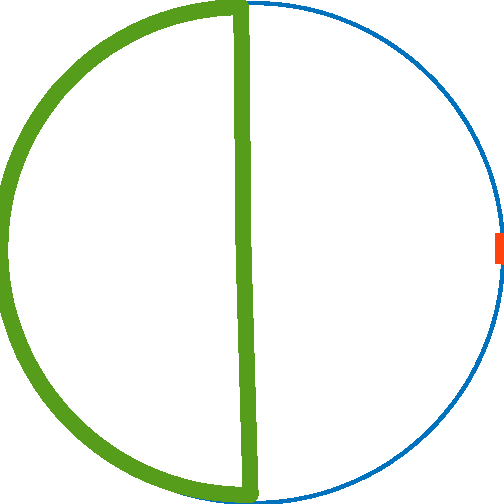
\includegraphics[width=2cm]{Pictures/1CAD_colored.pdf}};
		}
        \uncover<1->{
        \node [below =of N1,inner sep=0pt] [xshift=0cm,yshift=-0.9cm,inner sep=0pt](N5)
		{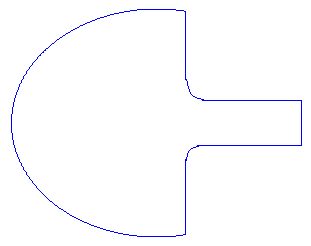
\includegraphics[width=2.2cm,height=2.2cm]{Pictures/End.png}};                        
		}        
        \uncover<1->{
       	\path[dashed,thick, ->,]<1-> (N1) edge [bend right] (N5) node[yshift=-2cm, xshift = -0.3cm]{User}; 
		 }     
        \uncover<2->{
        \node [right =of N1,inner sep=0pt] [xshift=1cm,yshift=-0cm, inner sep=0pt](N2)             
                {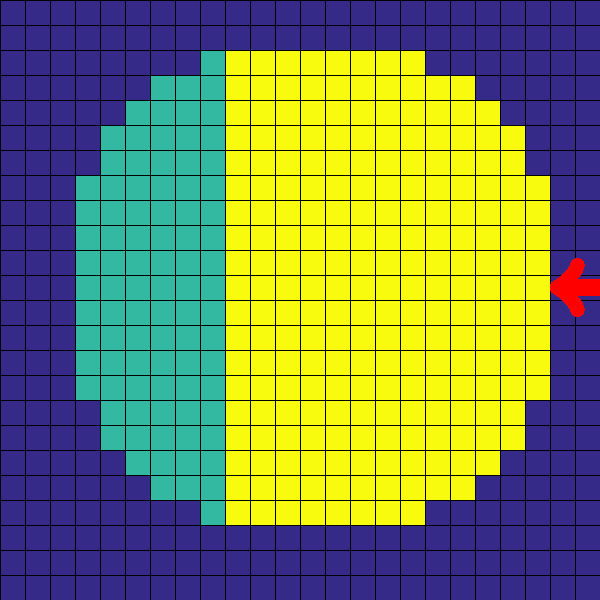
\includegraphics[width=2cm]{Pictures/4TPD.pdf}};
        \draw[thick,->] (N1) -- (N2);
        }
        \uncover<3->{
        \node [right =of N2,inner sep=0pt] [xshift=1cm,yshift=-2cm, inner sep=0pt](N3) 
                {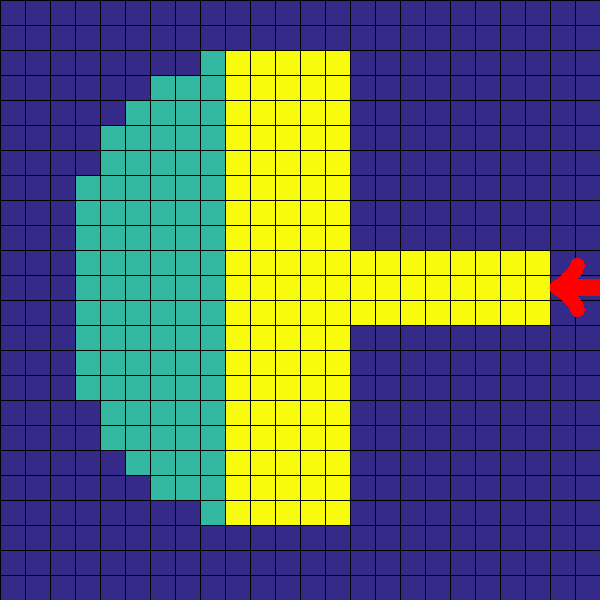
\includegraphics[width=2cm]{Pictures/5TOPOPT.pdf}};
        \draw[thick,->] (N2) -- (N3); 
        }
        \uncover<4->{
        \node [left =of N3,inner sep=0pt] [xshift=-1cm,yshift=-2.0cm, inner sep=0pt](N4)
                {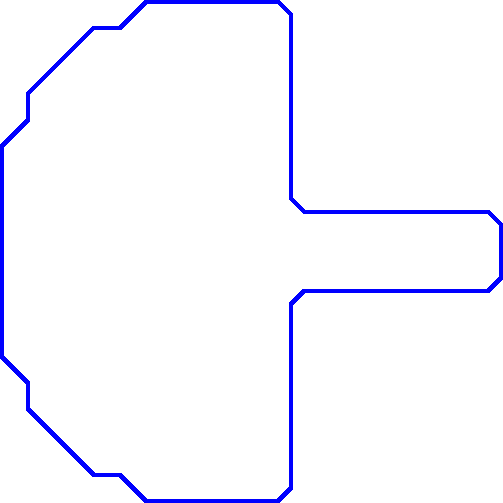
\includegraphics[width=2cm]{Pictures/7MC.pdf}};
        \draw[thick,->] (N3) -- (N4);
        }
        \uncover<5->{\draw[thick,->] (N4) -- (N5); 
        }
        \draw[red,thick,dotted] ($(N1.north west)+(-0.3,0.5)$)  rectangle ($(N5.south east)+(0.3,-0.4)$);
		\visible<1->{\node [above of=N1, yshift=0.2cm](Text1){CAD design};}
		\visible<2,6>{\node [above of=N2, yshift=0.2cm](Text2){Voxelized geometry};}
		\visible<3,6>{\node [above of=N3, yshift=0.2cm](Text3){Optimized topology};}
		\visible<4,6>{\node [below of=N4, yshift=-0.2cm](Text4){Extracted isosurface};}
		\visible<1->{\node [below of=N5, yshift=-0.2cm](Text5){B-Spline surface};}
        \end{tikzpicture}
	\end{center}
	\end{overlayarea}

\end{frame}
